\documentclass[
    pagesize,%         put paper size information into document (for ps and pdf!)
    a4paper,%          use a5paper for ISO A5; use a4paper for ISO A4
            %          adapt also pdf paper size!
%    BCOR12mm,%         set extra margin for book fixation
%    DIV11,%            set DIV for good linewidth explicitly
%    DIVcalc,%            typearea has to calculate DIV for good linewidth
    headsepline,%      use headinclude also! (see M. Kohm)
    footsepline,%      use footinclude also! (see M. Kohm)
    headinclude,%      count head to text body (not to margin) 
    footinclude,%      count foot to text body (not to margin) 
    bibtotoc,%         write bibliography-chapter to table of contents
%    idxtotoc,           % Stichwortverzeichnis ebenso
%    liststotoc,%       abbildungs- und tabellenverzeichnis ebenso
    cleardoubleplain,% \cleardoublepage generates pages with pagestyle plain
    tablecaptionabove,% setzt tabel caption besser ab 
%    final%            final version
%    draft%            draft version
]{scrreprt}



\usepackage[latin9]{inputenc}
\usepackage[english]{babel}
\usepackage[T1]{fontenc}

\usepackage{graphicx}
\usepackage{amsmath}
\usepackage{booktabs}
\usepackage{textcomp}
\usepackage{multirow}
\usepackage{color}
\usepackage{babelbib}
\usepackage{algpseudocode}
\usepackage{algorithm}
\usepackage{shadethm}

\usepackage{listings}

\usepackage{caption}
\usepackage{subcaption}
\usepackage{setspace}
\usepackage{booktabs}
\usepackage{gensymb}
\usepackage{pdflscape}
\usepackage{multirow}
\usepackage[table]{xcolor}
\usepackage{longtable}
%\usepackage[font={small,sf},format=plain,labelfont={bf,up}]{caption} %im text \textbf könnte raus
\usepackage{adjustbox}
\usepackage{etoolbox}
\usepackage[master,institut]{zfibmcover}        % load cover
\usepackage[sort,numbers]{natbib} % base bib style
\usepackage{tikz}
\usetikzlibrary{trees}

% The following package makes code look a little nicer, but it may not be present on all systems.
\IfFileExists{cmtt.sty}{\usepackage[override]{cmtt}}{}% better typewriter font
% \usepackage{ae}      % erzeuge lesbare Schriften in pdf (almost european
                       % font)




% ---------------------
% some default settings
% ---------------------

% caption font settings

\setkomafont{captionlabel}{\itshape\usekomafont{section}\footnotesize}
\setkomafont{caption}{\normalfont\scriptsize}

% Keine Serifenlose fuer description-Umgebungen
%
\renewcommand{\descfont}{\normalfont\bfseries}

% serifenlose und kleinere Schrift in Kopf und Fuss
\setkomafont{pagehead}{\normalcolor\sffamily\small}% what about \itshape?

\raggedbottom % Tanzender Fuss, tanzende fussnoten

\renewcommand{\cite}{\citep*}% change citation default command
\newcommand{\cites}{\citet*}% use for citation in sentence

%\bibpunct{(}{)}{;}{a}{}{,~} % configure citation style

\bibfont{\small} % smaller font for bibliography


\usepackage[NewCommands]{ragged2e} % overwrite old commands with new ones
\renewcommand*{\raggedsection}{\RaggedRight} % ragged right headings

% we want a flushleft bibliography (siehe typography rules)
\setbibpreamble{\RaggedRight}%

\setcounter{secnumdepth}{2} % Numerierung auch für \subsubsection
\setcounter{tocdepth}{1}    % nimm auch \subsubsections ins Inhaltsverz. auf


% Trennhinweise fuer Woerter hier beschreiben
%\hyphenation{
%}

%\usepackage[format=boldLabel]{caption}
%\DeclareCaptionFormat{boldLabel}{#3}

%Tabellen & Abbildungen des Anhang in Roemisch nummerieren
\newcommand{\beginsupplement}{%
	\setcounter{table}{0}
	\renewcommand{\thetable}{\Roman{table}}%
	\setcounter{figure}{0}
	\renewcommand{\thefigure}{\Roman{figure}}%
}

%use (a) for numbering subsections
%\renewcommand*\thesubsection{(\alph{subsection})}

\newshadetheorem{definitions}{Definition}[chapter]

\newenvironment{definition}[1][]{%
  \definecolor{shadethmcolor}{rgb}{.9,.9,.95}%
  \definecolor{shaderulecolor}{rgb}{0.0,0.0,0.4}%
  \setlength{\shadeboxrule}{1.5pt}%
  \begin{definitions}\hspace*{1mm}%
}{\end{definitions}}

\begin{document}

\Number{2014-01} % enter here the actual year and number of your thesis. 
\Title{Improving automatic task tree generation with alignment algorithms}
\Authors{Ralph Krimmel}
%\DepartmentType{}% use only if it is not "Lehrstuhl" or "Institut"
\Department{Institut f\"ur Informatik}

\Date{30.September 2014}

\areaset[1cm]{17cm}{27cm}% set format for cover page
\makecover

%\typearea[BCOR]{DIV}
%\typearea[10mm]{11}
\typearea{11}% set format for document


\pagestyle{headings}

\tableofcontents


\pagenumbering{arabic}
\setcounter{page}{3}


\clearpage
\chapter{Introduction}
\label{chap:introduction}

Task trees are a method to describe and structure the process of users interacting with software. 
The designer of the software can generate a task tree from the GUI model e.g. from HTML structure. In contradiction to the task trees generated at design time they can also be derived from recorded user actions. In this case, task trees offer the possibility to semi-automatically evaluate the usability of the software since it is then possible to compare expected with the actual user behaviour \citep{harms2013}.  

\begin{itemize}
	\item Definition of a task tree: type of task model which describe user actions
    	\begin{itemize}
		\item  e.g. used in Goals, Operators, Methods and Selection Rules (GOMS), TaskMODL and ConcurTastTrees (Zitat?)
	\end{itemize}
	\item Aim: analyze and compare effective and expected user interactions, semi-automatic usability evaluation
	\item two possible variants of task tree generation 
 	\begin{itemize}
		\item - generated from expected actions at design time
      		\begin{itemize}
			\item Tools/Software: Critique, ReverseAllUI (based on models of GUI) (sources...)
     			\item Problem: simplified or complete task tree
		\end{itemize}
		\item Actual user interactions (e.g. from event driven software)
     		\begin{itemize} 
			\item Programming by example: effective user actions recorded
			\item Problem: usability improved only on a local area
		\end{itemize}
	\end{itemize}
	\item Harms tries to get a more global view on software: usability could be improved by that (cite) 
	\item Disadvantages from harms method here!
	\item In this work I will cover the following aspects...
\end{itemize}


\section{Terminology}
	The basic building blocks of a task tree are ..
\begin{itemize} 
	
	\item Components of a task tree: (with picture)
	\begin{itemize}
		\item root node: represents the overall task which contains all subtasks, the user wants to "reach" this node by his actions/his input
		\begin{itemize}
    			\item Order something in a webshop
		\end{itemize}
		\item intermediate nodes: subtasks which are steps towards the overall task
		\begin{itemize}
			\item e.g.: create a new account/log in, put something into the basket
		\end{itemize}
		\item leaf nodes: actions (e.g. click, scroll, textinput) which cause an event (e.g. \textit{onclick} (click) or \textit{onchange} (textinput)
		\begin{itemize}
			\item e.g.: enter a product name in a text field and click on the "search"-button
		\end{itemize}
	\end{itemize}
	\item Where should i write about the difference between tasks and taskinstances? 	
	\item temporal relationship: the order of the executed actions is important, so it is saved in the task tree
	\item different ways of temporal relationship used by harms: 
	\begin{itemize}
		\item sequences: children executed in specific order
		\item iteration: only one child, executed zero or more times
		\item selection: only one of the children is executed
		\item optional:  only one child, executed once or not
	\end{itemize}	
	\item Trace: recorded sequence of events: monitoring module records events caused by user actions, stored 
	\item add example of a trace (maybe this goes to case study)
\end{itemize}
\section{Trace Based Task Tree Generation by Harms}
\begin{itemize}
	
	\item Procedure: start with leaf nodes to creat a task tree
 	\item for every event in a trace: crate an event task instance
  	\item event tasks instances stored in recorded order

	\item Iteration detection:
	\begin{itemize} 
		\item identical tasks, which often repeat directly (e.g.: click on the same button a few times): Iteration
		\item generate a new task model of type iteration: iterated event task as single child
		\item replace every occured iteration of the event task with the iteration task node 
	\end{itemize}

	\item Sequence detection:
	\begin{itemize}
		\item task list scanned for identical subsequences
    		\item most occured and longest subsequence: propably a logical and useful subtask
		\item new task node type sequence generated
		\item every identical subsequence replaced with the new task node 
		\item if same length and count of subsequence: first subsequence will be replaced (always only one subsequence replaced!
    		\item minimal length of a subsequence: 2 actions/ event tasks
	\end{itemize}
	\item Repetition of Detections:
	\begin{itemize}
		\item iteration and sequence detection repeatet until there are no matches anymore
  		\item replaced sequences may already contain iterations/sequences 
		\item in the end: list with task trees and event tasks that does not fit in as an iteration or sequence
		\item Problem: some event tasks are used only once (e.g. login) or very seldom by one user
		\item solution: compare data of more users 
	\end{itemize}
\end{itemize}


\clearpage
\chapter{Foundations}
\label{chap:foundations}
In this chapter we will provide and explain the concepts and terms that are used throughout this thesis. 
we will cover the definitions of a GUI and GUI-Model as well as the basic terminology of a task tree, followed by 
 information on alignment algorithms and substitution matrixes.
The last section describes the method for task tree generation by Harms et al.\cite{harms2013}


\section{GUI and GUI-Model}
\label{sec:foundationguiandguimodel}

TODO: GUI Model

\section{Task Tree Terminology}
\label{sec:foundationtasktreeterminology}
Harms et al.\cite{harms2013} have created a set of definitions and the respective vocabulary that help dealing with task trees.
We will adopt his definitions and summarize them in this section.

To understand tasks and task trees we have to look at how users interact with software. 
Users perfoming actions like clicking or typing trigger so called events. Those events consist of a type and a target. 
The type describes the type of the action that triggered that event (e.g. onclick), the target describes the element in the GUI the event occurred on.
The events a user creates can be traced which is the basic step to gather data that is needed to generate task trees. 
A trace is a list of events in the order they occurred. Table \ref{tab:trace} shows an example of such a trace. 
All events in this list and their corresponding actions represent the users intention to achieve a goal while using the software e.g. buying a book 
in an online shop. From now on this goal is named task. This task can consist of several subtasks such as logging in or putting a book into the basket.
Each subtask itself can again contain further subtasks. From figure \ref{fig:booktree} one can see this results in a tree structure, a so called trask tree.

\begin{table}
\begin{center}
 \begin{tabular}{l|l|l}
	   Order & Type & Target \\
	 \hline
	 \hline
	   1. & Left mouse button click &  Textfield with id username \\
	   2. & Text input "usr" &  Textfield with id username \\
	   3. & Left mouse button click &  Textfield with id username \\
	   4. & Text input "user" &  Textfield with id username \\
	   5. &Left mouse button click &  Textfield with id password \\
	   6. & Text input "" &  Textfield with id password \\
	   7. &Left mouse button click &  Button with name "login" \\
	  \end{tabular}
  \end{center}
  \label{tab:trace}
  \caption{Example for a trace of the login process of a user.\cite{harms2013}}
  \end{table}

\begin{figure}
	\tikzstyle{every node}=[rectangle, draw=none, rounded corners=1mm,
        text centered, anchor=west, text=black, fill=blue!30]
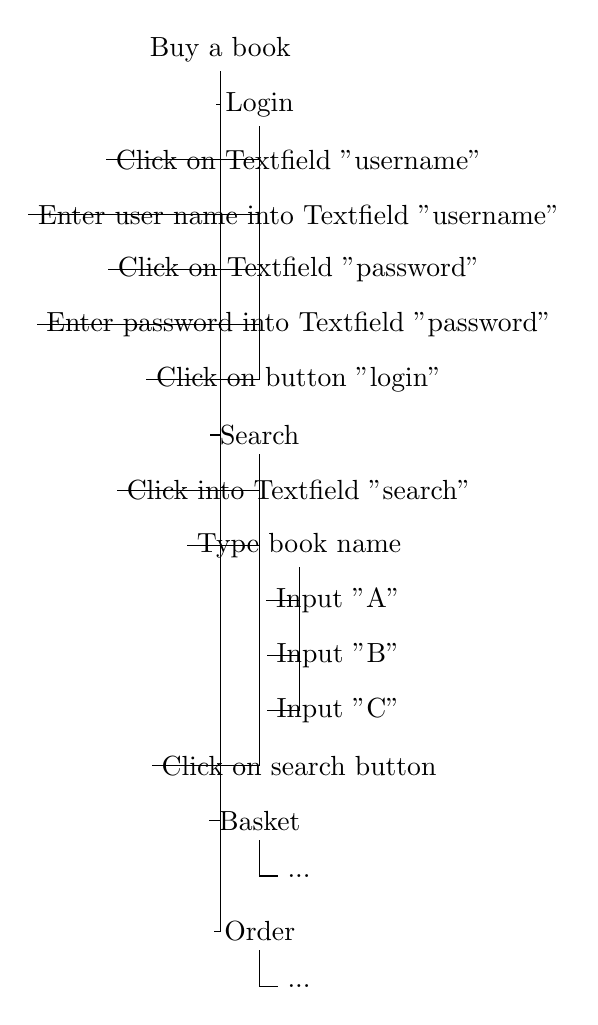
\begin{tikzpicture}[%
  grow via three points={one child at (0.5,-0.7) and
  two children at (0.5,-0.7) and (0.5,-1.4)},
  edge from parent path={(\tikzparentnode.south) |- (\tikzchildnode.west)}]

\node {Buy a book} [-]
    child{
        node {Login}
        child{ node {Click on Textfield "username"}}
        child{
            node {Enter user name into Textfield "username"}
        }
        child{
            node {Click on Textfield "password"}
        }
        child{
            node {Enter password  into Textfield "password"}
        }
        child{
            node {Click on button "login"}
        }
    }
    child [missing] {}
    child [missing] {}
    child [missing] {}
    child [missing] {}
    child [missing] {}
    child{
        node {Search}
        child{
            node {Click into Textfield "search"}
        }
        child{
            node {Type book name}
            child{
                node {Input "A"}
            }
            child{
                node {Input "B"}
            }
            child{
                node {Input "C"}
            }
        }
    child [missing] {}
    child [missing] {}
    child [missing] {}
        child{ node {Click on search button}}
    }
        child [missing] {}
        child [missing] {}
        child [missing] {}
        child [missing] {}
        child [missing] {}
        child [missing] {}
    child{ node {Basket}
        child{ node {...}}
    }
       child [missing] {}
    child{
        node {Order}
        child{ node {...}}
    }
;
\end{tikzpicture}

	\label{fig:booktree}
	\caption{Simplified and not complete visit of an online book shop as a task tree}
\end{figure}

A task tree consists of three different kinds of nodes:
\begin{itemize} 
	\item Root node: Represents the overall task which contains all subtasks, the user wants to achieve this goal by his actions/his input. 
		In figure \ref{fig:booktree} the overall task is to buy books at an online shop.
	\item Intermediate nodes: Are subtasks which are steps towards the overall task. In figure \ref{fig:booktree} the intermediate nodes are login, search, basket and order.
	\item Leaf nodes: Actions (e.g. clicking, scrolling, textinput) which cause an event (e.g. \textit{onclick} (click) or \textit{onchange} (textinput). The tasks at this level are called event tasks. Event tasks have no further children. Some events tasks of \ref{fig:booktree} are for example Input A, Input B and Input C.
\end{itemize}
Another relevant point is that the order of the executed actions is important. Therefore this information has to be represented in the task tree as well. For this Harms et al. defined the so called temporal relationships for all non-event-tasks. There are four types of temporal relationships, each with different properties. The \textit{sequence} temporal relationship dictates that children have to be executed in specific order to fulfil the task. An \textit{iteration} can just have one child which is executed once or more times. Just one child of a \textit{selection} is allowed to be executed whereas the one child of an \textit{optional} may or may not be executed. Figure \ref{fig:exampletasktree} shows a tasktree that represents a login procedure and contains all possible temporal relationships. At last Harms et al. differentiate between a task and an executed task, a task instance. Figure \ref{fig:exampletaskinstancetree} shows the main differences between a task and its instance: \textit{Selection} instances can have only one child with the task instance that was executed. \textit{Optional} instances have one child if the task was executed and none if not. Instances of \textit{iterations} have as many children as often the task was executed.
	\begin{figure}
		\tikzstyle{every node}=[rectangle, draw=none, rounded corners=1mm,
		        text centered, anchor=west, text=black, fill=blue!30]
		
		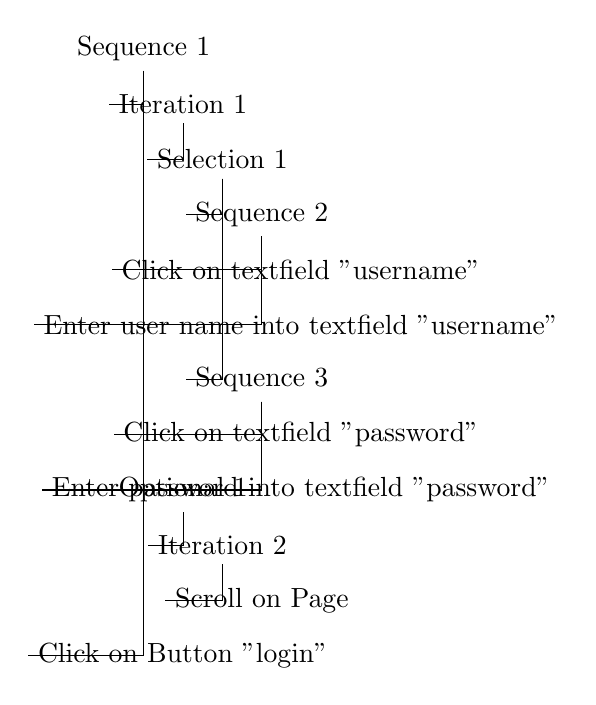
\begin{tikzpicture}[%
		  grow via three points={one child at (0.5,-0.7) and
		  two children at (0.5,-0.7) and (0.5,-1.4)},
		  edge from parent path={(\tikzparentnode.south) |- (\tikzchildnode.west)}]
		  \node {Sequence 1}
		    child { node {Iteration 1}       
		      child { node {Selection 1}
		        child { node {Sequence 2}
				child { node {Click        on   textfield "username"}}
		          child { node {Enter user name    into textfield "username"}}
		      child [missing] {}
		          child [missing] {}
		    }
		        child [missing] {}
		    child [missing] {}
		        child { node {Sequence 3}
		          child { node {Click        on   textfield "password"}}
		          child { node {Enter password  into textfield "password"}}
		        }
		      }
		    }
		    child [missing] {}
		    child [missing] {}
		    child [missing] {}
		    child [missing] {}
		    child [missing] {}
		    child [missing] {}
		    child { node {Optional 1}
			    child { node {Iteration 2}
				child{ node{Scroll on Page}}
			}
		    }
		    child [missing] {}
		    child [missing] {}
		    child { node {Click        on   Button "login"}};
		    \end{tikzpicture}
		\label{fig:exampletasktree}
		\caption{An example for a task tree with temporal relations\cite{harms2013}.TODO: More explanations here}
	\end{figure}
	\begin{figure}
		\tikzstyle{every node}=[rectangle, draw=none, rounded corners=1mm,
		        text centered, anchor=west, text=black, fill=green!30]
		
		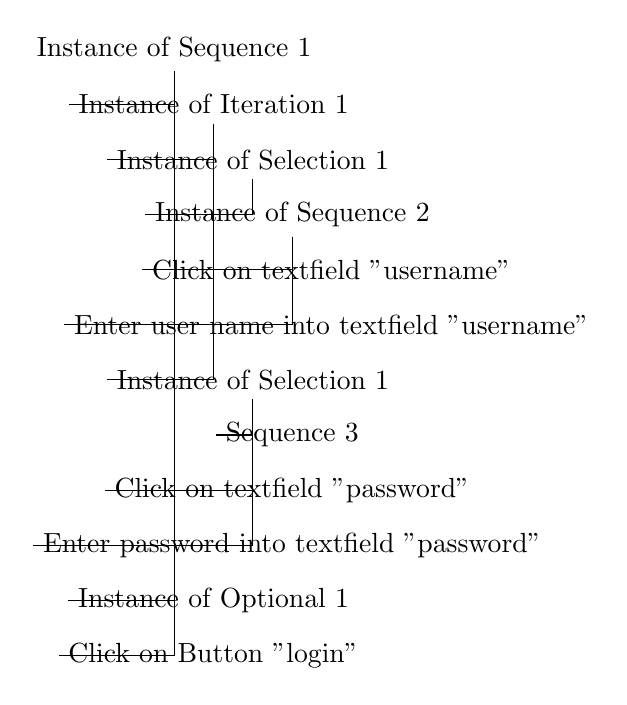
\begin{tikzpicture}[%
		  grow via three points={one child at (0.5,-0.7) and
		  two children at (0.5,-0.7) and (0.5,-1.4)},
		  edge from parent path={(\tikzparentnode.south) |- (\tikzchildnode.west)}]
		  \node {Instance of Sequence 1}
		    child { node {Instance of Iteration 1}       
		      child { node { Instance of Selection 1}
		        child { node { Instance of Sequence 2}
			  child { node {Click        on   textfield "username"}}
		          child { node {Enter user name    into textfield "username"}}
		          child [missing] {}
		          child [missing] {}
		        }
		      }
		      child [missing] {}
		      child [missing] {}
		      child [missing] {}
		      child { node { Instance of Selection 1} 
			  child { node {Sequence 3}}
		          child { node {Click        on   textfield "password"}}
		          child { node {Enter password  into textfield "password"}}
		       }
	            }	
		    child [missing] {}
		    child [missing] {}
		    child [missing] {}
		    child [missing] {}
		    child [missing] {}
		    child [missing] {}
		    child [missing] {}
		    child [missing] {}
		    child { node { Instance of Optional 1}} 
		    child { node {Click        on   Button "login"}};
		    \end{tikzpicture}
		\label{fig:exampletaskinstancetree}
		\caption{An example for one task tree instance of the task tree in figure \ref{fig:exampletasktree}\cite{harms2013}.}
	\end{figure}
\section{Alignments}
Alignments are a method in bioinformatics to compare strings or sequences of DNA/RNA/Amino acids and score their similarity. 
It is a very basic task to find out if two sequences are related. 
This is done by arranging those sequences in a way that similar elements of each sequence are aligned together. The biological background of this approach is that
both sequences have diverged from a common ancestor by a process of mutation and selection\cite{durbin1998}, hence have still common regions. The differences between those
sequences can be explained by three processes: \textit{Substitution} which replaces one element with an other,  \textit{deletion} which removes an element and \textit{insertion} that adds a new element to a sequence.
Both insertion and deletion produce a so called gap in the alignment since the change just appeared in one of the two aligned sequences. Figure \ref{fig:alignmentbasic} illustrates all possible modifications.
Each modification can be scored individually but it is common practise to score substitutions with substitution matrixes and have a general gap penalty. The sum of all single scores is the score of the total alignmment.
Alignment algorithms try to maximize this score.

\begin{figure}[h]
	\centering
	\begin{subfigure}[b]{0.3\textwidth}
	\begin{tabular}{c|cccc}
		1: &A&B&C&D\\
		2: &A&B&C&A\\
	\end{tabular}
	\caption{Subsitution of D} 
	\end{subfigure}
	\begin{subfigure}[b]{0.3\textwidth}
	\begin{tabular}{c|cccc}
		1:&A&B&C&D\\
		2:&A&B&-&D\\
	\end{tabular}
	\caption{Deletion of C} 
	\end{subfigure}
	\begin{subfigure}[b]{0.3\textwidth}
	\begin{tabular}{c|cccc}
		1:&A&B&C&-\\
		2:&A&B&C&D\\
	\end{tabular}
	\caption{Insertion of D}
	\end{subfigure}
	\label{fig:alignmentbasic}
	\caption{Three possible modifications that can occurr to sequence 2}
\end{figure}

Alignments can be categorized into global and local alignments. Global alignment algorithms try match one sequence to the other from start to end whereas local alignment algorithm try to find the best alignment of subsequences. 
A popular global alignment algorithm is the Needleman-Wunsch algorithm\cite{needleman1970}. For basic local alignments the common algorithm is from Smith and Waterman\cite{waterman1981}.

\section{Substitution Matrixes}
\label{sec:foundationsubstitutionmatrix}
In the last section I stated that alignment algorithms maximize the total alignment score. Therefore the underlying scoring model has to be adjusted very carefully since it practically determines the outcome of the algorithm.
There are usually two parameters which have to be set: the substitution score and the gap penalty. 

The gap penalty in its most basic version is a constant that has to be manually adjusted so that it fits the problem well. 
A large gap penalty leads to less insertion and deletion occurrence and more substitutions.
This gap scoring is called linear affine gap penalty. (TODO: Cite)
The total gap penalty is n*g with n being the number of gaps and g the gap penalty constant. 
There are different gap penalty models like a different g for opening a new gap and extending an already open gap. 
In this thesis I will just use the linear affine gap penalty. 

The substitution score is a representation of how similar two elements are. The more similar they are, the higher the score will be.
The score is usually stored in symmetric matrices where each cell represents how good or bad it is to substitute element a with element b. 
%In biology 
%	In Biology popular matrices are generated from real DNA data (PAM, BLOSUM) (cite)
\begin{figure}
	\label{fig:submatexample}
\end{figure}

\section{State of the Art of Trace Based Task Tree Generation}
\begin{itemize}
	\item Procedure: start with leaf nodes to creat a task tree
 	\item for every event in a trace: create an event task instance
  	\item event tasks instances stored in recorded order

	\item Iteration detection:
	\begin{itemize} 
		\item identical tasks, which often repeat directly (e.g.: click on the same button a few times): Iteration
		\item generate a new task model of type iteration: iterated event task as single child
		\item replace every occured iteration of the event task with the iteration task node 
	\end{itemize}

	\item Sequence detection:
	\begin{itemize}
		\item task list scanned for identical subsequences
    		\item most occured and longest subsequence: propably a logical and useful subtask
		\item new task node type sequence generated
		\item every identical subsequence replaced with the new task node 
		\item if same length and count of subsequence: first subsequence will be replaced (always only one subsequence replaced!
    		\item minimal length of a subsequence: 2 actions/ event tasks
	\end{itemize}
	\item Repetition of Detections:
	\begin{itemize}
		\item iteration and sequence detection repeatet until there are no matches anymore
  		\item replaced sequences may already contain iterations/sequences 
		\item in the end: list with task trees and event tasks that does not fit in as an iteration or sequence
		\item Problem: some event tasks are used only once (e.g. login) or very seldom by one user
		\item solution: compare data of more users 
	\end{itemize}
\end{itemize}


\chapter{Approach}
\label{chap:approach}
The algorithm proposed by Harms is well designed but is not capable of finding similar user sequences. 
When there is more than one possible interaction to achieve a goal, the method of Harms will create two different sequences for that interaction, 
or worse, will not detect the interaction as a meaningful one at all. For this reason I propose an algorithm that is able to detect similar subsequences.
The basic steps of the algorithm do not differ alot from Harms one. In fact some preprocessing steps and the sequence detection have been altered.
Algorithm \ref{alg:tasktreeoverview} shows the main building blocks and will function as a list and order of contents of this chapter.
\section{Task Tree Generation}

\begin{algorithm}[h]
\floatname{algorithm}{Algorithm}
\begin{algorithmic}
	\Procedure{GenerateTaskTree}{UserSessions}
	\State Generate Substitution Matrix (UniqueTasks)
	\While{Replaced Tasks} 
	\State Detect Iterations (UserSessions)
	\State Optional: Substitution Matrix Update
	\State Detect Sequences (UserSessions,SubstitutionMatrix)
	\EndWhile
	\EndProcedure
\end{algorithmic}
\caption{Overview over the task tree generation}
\label{alg:tasktreeoverview}
\end{algorithm}

\section{Task Distance Substitution Matrix}
The harmonization process performed by Harms et al. is also applied to the user sessios in this approach. 
A useful side product of the harmonization is the set of unique tasks.
This set is needed for this step of the algorithm, the generation of the substitution matrix.

In section \ref{sec:foundationsubstitutionmatrix} we introduced substitution matrixes in general and what they are good for. 
For this use case we needed to generate one substitution matrix that represents how similar tasks are. 
The score of two tasks in the \textit{task distance substitution matrix} is defined as follows:
\begin{definition}
	\item Let a and b be two tasks
	\item Let S(a,b) be the score for substituting task a with task b. The higher the value of S is, the more similar are the tasks a and b and vice versa.
\end{definition}

To calculate the score, three cases have to be considered:
\begin{itemize}
	\item Similarity of two event-tasks
	\item Similarity of an event-task and a non-event-task
	\item Similarity of two non-event-tasks
\end{itemize}

\subsection{Event-Task Event-Task Similarity}
The first idea was to calculate the score of the matrix based on the distance between the absolute coordinates of the events-tasks. 
There are a few problems with this approach: First, not all event-tasks may have absolute coordinates. 
The second problem with this method is that in graphical user interfaces events may still be very similar, even if they have a large absolute distance.
An example for such a case would be a web formular with many fields to fill out. 
TODO: Maybe Screenshot here?
Those fields take space which would result in large distances between them although the event-tasks all belong to a single formular.
The solution to this problems is to make use of a grouping of elements the designer of the GUI already did: The GUI-Model (see section \ref{sec:foundationguiandguimodel}).
Elements of a GUI that belong to one semantic task can usually be found in some kind of container that groups those elements together. Therefore the basis for my 
distance calculation is the distance in the GUI-Model, as defined in \ref{def:guimodeldistanceee}. 

\begin{definition}
	\item Let a and b be events-tasks
\begin{equation*}d(a,b) = d(b,a) = \text{the distance in the GUI model of the targets of event-tasks a and b.}
\end{equation*}
\label{def:guimodeldistanceee}
\end{definition}

Since the GUI model is a tree, the distance of two targets in a GUI can easily be calculated by finding the common ancestor of the targets and summing up the number of nodes from both the events to this ancestor, including the ancestor.
\begin{figure}
\begin{center}
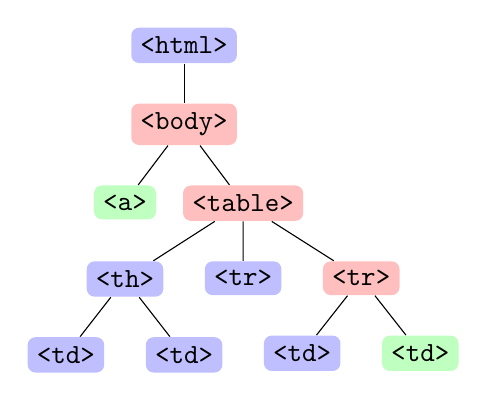
\begin{tikzpicture}[
    fact/.style={rectangle, draw=none, rounded corners=1mm,
        text centered, anchor=north, text=black, fill=blue!25},
    redcolor/.style={rectangle, draw=none, rounded corners=1mm,
        text centered, anchor=north, text=black, fill=red!25},
    greencolor/.style={rectangle, draw=none, rounded corners=1mm,
        text centered, anchor=north, text=black, fill=green!25},
    level distance=0.5cm, growth parent anchor=south]

\node (Fact01) [fact] {\texttt{<html>}} [-]
    child{
        node (kolor4) [redcolor] {\texttt{<body>}}
        child{
            node (color1) [greencolor] {\texttt{<a>}}
        }
        child{
            node (Fact04) [redcolor] {\texttt{<table>}}
            child{
                node (Fact05) [fact] {\texttt{<th>}}
                child{
                    node (fact5) [fact] {\texttt{<td>}}
                }
                child{
                    node (Fact07) [fact] {\texttt{<td>}}
                }
            }
	    child{
                node (Fact05) [fact] {\texttt{<tr>}}
	    }	
            child{
                node (color3) [redcolor] {\texttt{<tr>}}
                child{
                    node (Fact10) [fact] {\texttt{<td>}}
                }
                child{
                    node (color2) [greencolor] {\texttt{<td>}}
                }
            }
        }
    }   
;
 
\end{tikzpicture}
\end{center}	
\label{fig:guimodeldistance}
\caption{A HTML GUI model with two nodes (green) the distance will be calculated for.  The number of red nodes is the distance between the green nodes. The common anchestor is the \texttt{<body>} element.}

\end{figure}
Figure \ref{fig:guimodeldistance} shows a GUI model with two elements and their common ancestor. 


\subsection{Event-Task Non-Event-Task Similarity}
It takes a bit more effort to calculate the substitution score if one task is a non-event-task. 
The reason is that the non-event tasks do not represent a simple event anymore. Therefore they do not possess a target in the GUI.
A possible solution is to recursively visit every child of the non-event-task, gather all event tasks and then calculate the mean distance from each of those tasks to the event-task the distance shall be calculated to.
Formally, definition \ref{def:guimodeldistanceee} has to be modified so that it covers non-events as well:

\begin{definition}
%	\item Let a and b be events-tasks, then:
%\begin{equation*}d(a,b) = d(b,a) = \text{be the distance in the GUI model of the targets of event-tasks a and b.}
%\end{equation*}
	\item Let c be a non-event-task
	\item Let E be the set containing all event-tasks that can be recursively found in c.
	\item with definition \ref{def:guimodeldistanceee} it is possible to define d as
\begin{equation*}
	d(a,c) = d(c,a) = \frac{\sum_{\forall x \in E} d(a,x)}{|E|}
\end{equation*}
\label{def:guimodeldistanceene}
\end{definition}

\subsection{Non-Event Non-Event Similarity}
With Definition \ref{def:guimodeldistanceene} it is simple to compute the distance for two tasks since all that is to do now is to repeat the procedure of finding all event-task children of one task, calculate the distances to the other task and use the mean distances as the total distance.
The definition of d can be extended so it accepts two non-event-tasks:

\begin{definition}
	\item Let c and d be non-event-tasks 
	\item Let E be the set containing all event-tasks that can be recursively found in c.
	%\item Let F be the set containing all event-tasks that can be recursively found in d.
	\item with definition \ref{def:guimodeldistanceene} it is possible to define d as
	\begin{equation*}
		d(c,d) = d(d,c) = \frac{\sum_{\forall x \in E} d(x,d)}{|E|}
	\end{equation*}
\label{def:guimodeldistancenene}
\end{definition}
\subsection{Score}
Now that I defined the distance for three cases it is possible to compute the score $S$ of two tasks.
\begin{definition}
	\item Let U be the set of unique tasks occurring in the user sessions
	\item Let k be a constant that defines the maximal score 
	\item For each tupel $i,j \in U$ 
\begin{equation*}
		 S(i,j) = -1*d(i,j)+k
	\label{eq:subscore}
\end{equation*}
\end{definition}

The k constant should be chosen dependent on the underlying GUI model. A large k should be chosen for very deeply, nested GUI models whereas for flat GUI models a smaller k seems better. 

The maximal score is reached if the distance between two elements is zero. This happens if we compare two equal elements.
A problem can occur when the score of a non-event-task to an event task is equal to maximal score. 
This happens if a non-event-task has just one event-task as child and the distance of this child to the same event-task is calculated. 
Since it is preferred that the score of two equal event-tasks is always larger than the score of this event-task with a non-event-task we add the penalty term $L$ to the score equation.

\begin{definition}
	\item Let E be the set of all event-tasks
	\item let N be the set of all non-event-tasks
\begin{eqnarray*}
	L(i,j) &=& 
	\begin{cases}
		0 & \text{if } i,j \in E \\
		\text{constant} & \text{if } i \in N \lor  j \in N\\
	\end{cases} \\
	S(i,j) &=& -1*d(i,j)+k-L
\end{eqnarray*}
	\label{eq:subscore_adjusted}
\end{definition}


\section{Iteration Detection and Substitution Matrix Update}
The iteration detection from Harms is also suitable for my algorithm was not altered in any way. It reliably detects iterations and replaces them in the user sessions.
Before the sequence detection can come to play the substitution matrix should be updated since there were new iteration tasks created during iteration detection. Those new tasks are stored in a set that contains all newly created tasks.
The update process differs just a little from the generation process with the only difference beeing that just the distances between the newly created tasks to the current set of unique tasks is as well as the distances between the newly created tasks are computed.
After the matrix has been updated, the newly created tasks are merged with the set of unique tasks and then emptied.
TODO: NOT UP TO DATE The whole step of updating the matrix is currently implemented but not used. 
Instead, each score between an event-task to a non-event-task and therefore all scores between non-event-tasks are defined as zero due to perfomance issues.
More details on this issue can be found in section TODO: REF HERE.

\section{Sequence Detection}
As we figured out at the beginning of this chapter the sequence detection is the part of the algorithm that varies the most from Harms approach.
It is itself separated in three steps:
\begin{itemize}
	\item The search for significant patterns
	\item The model generation
	\item The sequence replacement
\end{itemize}

\subsection{Search for significant patterns}		
The search for significant patterns is done with an alignment method we introduced in section \ref{sec:alignments}. 
The bioinformatical problem of comparing and aligning DNA/RNA/Amino acid sequences is closely related to finding important subsequences in the user sessions. 
The conserved regions of biological sequences comply with those interactions that most of the users performed similarly. 
We can conclude that those interactions are meaningful in the sense of fulfilling one desired task.
The goal of the alignment algorithm is now to detect the conserved regions and extract a model of the average user behaviour. 
Since alignment algorithms also find approximate and not only exact similarities, this step of the sequence detection is the main difference to Harms method.

The first step of the search for significant patterns is to align every user session with any other user session with an algorithm called Smith-Waterman algorithm for repeated matches.
For the rest of this section the user session will be represented by a sequence of numbers. Each number in a sequence corresponds with the unique id the task at this position in the user sessions has.
We now describe the algignment algorithm in detail.

\paragraph{Smith Waterman Algorithm For Repeated Matches}
The Smith-Waterman algorithm for repeated matches\cite{durbin1998} is a modified version of the original Smith-Waterman algorithm\cite{waterman1981}.
The original Smith-Waterman finds the best local similarity between two sequences.
Since we need all relevant similarities and not just the one with the best score, we define a threshold score $T$.
Once a local subalignment reaches T it is considered as relevant.

We recall from the alignments introduction that alignment algorithms try to find the best possible score between two sequences using the underlying scoring model of substitution and gap scores.
The most na\"ive approach is to try out all possible combinations both sequences could be aligned. As usual, this approach is not very feasible because there are 
\begin{equation*}
	\binom{2n}{n} = \frac{(2n)!}{(n!)^2} \simeq \frac{2^{2n}}{\sqrt{\pi n}}
\end{equation*}
possible global alignments of two sequences\cite{durbin1998}. 
Another way would be to use some kind of heuristic but we are interested in an exact, deterministic method.
A common technique to solve this issue is dynamic programming\cite{bellman1957}. 
The main idea of dynamic programming is not to calculate every possible variant but to reuse the best solutions of smaller subproblems.  
This method is central to computational sequence analysis\cite{durbin1998}.

\subparagraph{Basic Smith-Waterman}
The basic version of the Smith-Waterman algorithm makes use of dynamic programming by defining the dynamic programming matrix $F$ where each cell of the matrix stores the best score for aligning the elements up to the position the cell represents.
For example the cell $(2|2)$ stores the score for the best alignment of first two elements of each sequence. 
Each cell is computed by getting the best score out of four choices. Prior to enlisting those, we need the following definitions: 

\begin{definition}
	\item Let x,y be two sequences
	\item Let F be a matrix with F(i,j) being the best score of aligning $x_1\dots x_i$ with $y_1\dots y_j$
\end{definition}

Then we can compute F by repeatedly applying the following equation:
\begin{equation}
F(i,j) = max \left\{ \begin{array}{lr}0,&\\F(i-1,j-1)+S(x_i,y_j),&Substitution\\F(i-1,j)-g,&Gap\\F(i,j-1)-g.&Gap\\\end{array} \right. 
\end{equation}
Figure \ref{fig:basicalignmentoperations} illustrates this formula. The diagonal choice means we align one element from each sequence with each other. Therefore we have to look up the similarity of both elements in the substitution matrix. 
When the score from the upper cell minus the gap penalty is bigger than the diagonal choice a gap will appear at this position in sequence y. 
This is the same for when the option from the left cell is taken, just that the gap will be inserted in sequence x. 
The option 0 in the equation is to prevent alignment scores to become negative. 
If a match cannot be extended with its score being a positive value it is better to start a new one later. 
As we can see it is possible to fill the whole matrix by once the trivial scores, the first row and the first column, have been initialized.

\begin{figure}
	\centering
	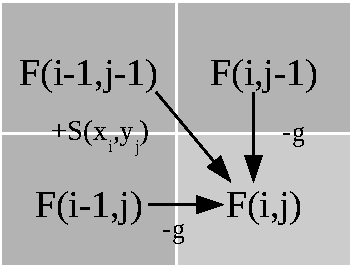
\includegraphics{img/basic_cell_fill.pdf}
	\caption{Illustration of the three operations deletion, insertion and substitution in a dynamic programming matrix}
	\label{fig:basicalignmentoperations}
\end{figure}

\subparagraph{Repeated matches}
In the improved version of the algorithm a cell in F has a slight different meaning and its computation is a bit more complex. 
The first difference is that this algorithm is asymetric in the sense of aligning sequence x to sequence y produces a different outcome than aligning sequence y to sequence x. Hence, we define y as the pattern we want to search and x as the sequence in which we search all subsequences of y repeatedly.
This results in a final alignment where x has matched and unmatched regions.  

The algorithm itself is partitioned into three parts: 

\begin{itemize}
	\item Initialization
	\item Recursion
	\item Traceback
\end{itemize}

\subparagraph{Intialization:}
	The initialization step is simple: \\
	Let m be the length of y
	
	\begin{equation*}
		F(0,j) = 0 \text{ for } j=0\dotsc m
	\end{equation*}
	This differs from the Smith-Waterman algorithm described by Durbin et al.\cite{durbin1998} who just initialize F(0,0) and do not fill the first column. There is no need to initialize the first row because a subalignment will never start with a gap. For the sake of an easy implementation it was better to initialize the first row though.

\subparagraph{Recursion}
The recursion formula for filling the matrix also has the three options for insertion/deletion and substitution as illustrated in figure \ref{fig:basicalignmentoperations}.
But as we see there are some more options. 
For the first row (equation \ref{eq:firstrow}), which does not represent a real alignment of sequences but denotes the sum of completed match scores, we have two options. 
The first one is to take the the the value from the last column so we always keep track of the total score. 
This leads to the fact that the value in this line will always stay the same or increase, but never decrease.
The second choice is taken when a match reaches its maximum and has a minimum score of T. 
This is the consequence of an ending match meaning this choice is just taken when we calculate the cell for an unmatched region.
To summarize the equation for the first row we can say the algorithm choses the maximum value of the last column minus T or adopts the value of the preceding cell in the first row, depending which one was larger. 

Equation \ref{eq:otherrows} for the fields aside of the first row is amended by the posibility to begin its alignment score with the value standing in the first row of its own column. 
Durbin et al. does not mention the fact that this makes it easier for subalignments of long sequences to reach the threshold score once a few matches have been found before.
This issue has not been investigated in this work. 
The total score of the whole alignment is stored in F(i+1,0). This cell lies an unmatched region of x and contains the sum of all completed match scores.


\begin{equation}
F(i,0) = max \left\{ \begin{array}{lr}F(i-1,0),&\\F(i-1,j)-T,& j=1,\dots,m\end{array}\right. 
\label{eq:firstrow}
\end{equation}
\begin{equation}
F(i,j) = max \left\{ \begin{array}{lr}F(i,0),\\F(i-1,j-1)+S(x_i,y_i),\\F(i-1,j)-g,\\F(i,j-1)-g.\end{array}\right.
\label{eq:otherrows}
\end{equation}
		
\subparagraph{Traceback}
A very important point in dynamic programming algorithms is that we not just calculate and store the maximum score for each subalignment but additionally have to store which choice of the formula produced the highest value.
This makes it possible to go back from the total best score to the start and find the actual alignment of the whole sequences. This process is called traceback. 
Figure \ref{fig:durbindpmatrixtraceback} shows a completly filled dynamic programmic matrix and the traceback path.

\begin{figure}
\centering
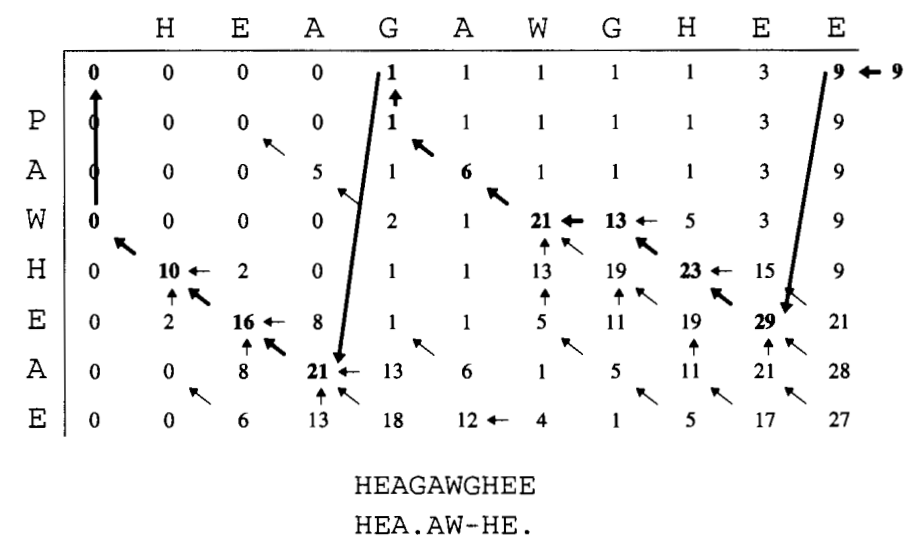
\includegraphics[scale=0.4]{chapters/approach/smithwatermanrepeated.png}
\caption{Figure from Durbin et al.\cite{durbin1998}. The repeat dynamic programming matrix for two example sequences, for T = 20. Below the optimal alignment, with total score $9 = 29-20$. There are two separate match regions, with scores 1 and 8. Dots are used to indoicate unmatched regions of x. The arrows show the traceback process, going back from the total score to the start.}
\label{fig:durbindpmatrixtraceback}
\end{figure}

\subparagraph{Match retrival}
To find similar user behaviour we are just interested in the matches that reached the threshold score. After aligning every user session with each other we extract all matches from those alignments.
We consider every subset of the alignment that is not a unmatched region a match.
Therefore a match consists of two sequences of numbers and can contain gaps. We will encode a gap in the number -1. 
Fig \ref{fig:matchexample} shows an example of a match, containing one gap in the first sequence, two exact tasks and one substitution.


\begin{figure}[h]
	\centering
	\begin{tabular}{cccc}
		9 & 16 & -1 & 6 \\
		9 & 15 & 17 & 6  
	\end{tabular}
	\caption{Example for a retrieved match}
	\label{fig:matchexample}
\end{figure}
	\begin{itemize}
		\item Search match in all user sessions
		\item From the most to the least found match:
	\end{itemize}
\subsubsection{Model generation}
	\begin{itemize}
		\item Generate Model From Match is done the following way:
		\item For each position of the Match: 
		\item (remind, that each match has 2 Sequences of aligned numbers)
		\begin{itemize}
			\item If Both numbers are equal: The model at this position is the Task refered by this number
			\item If one sequence has a gap at this position: The other EventTask is inserted as an optional
			\item If both numbers differ a selection is inserted. Which kind of selection depends on what the following task is. We don't want to have 2 selections next to each other, instead, create one selection and add each sequence as a sequence
			\begin{itemize}
				\item If the next position also would be a selection, the selection has 2 sequences as a child. those sequences consists of the tasks of each sequence of the match until there is no more selection found 
				\item If the next position is something else we just have a single selection, just add the tasks of the match at this position as childs to the selection
				\item (This description here is really bad, will need some examples)
			\end{itemize}
		\end{itemize}
	\end{itemize}

\subsubsection{Replacement}
	\begin{itemize}
		\item Replace each model in the user sessions
	\end{itemize}

\subsection{Repetition}





\clearpage
\chapter{Implementation}
\label{chap:implementation}

S. Herbold and P. Harms implemented their approach in the proof of concept implementation AutoQUEST.
AutoQUEST \textit{"provides diverse methods for assessing the quality
of software. AutoQUESTs internal algorithms operate on
abstract events, which makes AutoQUEST independent of
the platform of an assessed software"} \cite{herbold2013}. 
Another feature of AutoQUEST is that it is modular and extensible via plugins.
AutoQUEST is written in Java 1.7 and is published and licensed under the Apache License Version 2.0\footnote{http://www.apache.org/licenses/LICENSE-2.0.html}.
In this chapter we will document how we extended AutoQUEST by our task tree generation method.

%The most time spent developing for AutoQUEST was to get eclipse running.
The alignment sequence detection was implemented in one subversion branch of the autoquest-core-tasktree package. 
In AutoQUEST this module is responsible for the task tree generation. 
The most issues we had to solve existed due to the complexity of the problem, which is \textit{O}$(n^2)$ for most of the utilized algorithms.

\section{Substitution Matrix}
\subsection{Generation}
The generation of the substitution matrix is a step we just need to do once at the beginning of the sequence detection.
For a reasonable number of unique tasks no problems were expected but for a large number an efficient storage had to be implemented.
Since the substitution matrix is symmetrical it is common practise to just store \begin{equation*} \frac{n(n+1)}{2}\end{equation*} entries and not the whole matrix. 
Another improvement is that just a single array of primitive floats has been used which saves space again, namely \texttt{n} times the size of a float array.
The generation of the substitution matrix is so far not parallelized but it is possible to do so. 
The calculation of one cell in the matrix is nearly completly indepedent from another cell. 
This would save further time, given enough processors.


\subsection{Updating}
	The procedure of updating the substitution matrix is implemented but has just been tested on a very small data set. 
	Since the Matrix grows with \textit{O}$(n*(n+1)/2)$ for large data sets the calculation of non event-tasks is switched off because each generated task increases \texttt{n}.
	Also, the computation of non-event-tasks is complex itself. 
	First, for each task all event-tasks have to be searched. This is done by implementing the visitor pattern. 
	Then for each found event-task distances have to be calculated or read from the substitution matrix.
	To solve the issue of retrieving the event-tasks for each task again they are stored to hav
	This process could as well be parallelized but still, storing in the matrix has to be synchronous. 
	Another point is when the matrix is updated, its size has to be enlarged. 
	We could not use dynamic structures like the Java Collection ArrayList because its memory consumption becomes very inefficient when storing a large number of 
	float values. The solution was to keep using simple arrays and reserve more memory than initialy needed.
	So if the substitution matrix update is switched on, the matrix preallocates 10 times the initial unique tasks and doubles each time the size limit is reached.
	This increase of the size is very expensive since the whole matrix has to be copied to the newly created, larger sized matrix.

\section{Alignments}
Currently available and popular alignment tools are usually developed for the use in a biological context. 
The problem with these is that those tools are just working on sequences with a limited alphabet like the bases in DNA (A,C,T,G), RNA (A,C,U,G) or polypeptides (alphabet size 20).
Because of this issue we could not reuse well tested implementations of common or more complex algorithms. 

The Smith Waterman algorithm and its modified version are \textit{O}$(n^2)$ algorithms with \texttt{n} being the length the sequences being aligned.
This may not be an issue because the user session itself may not be too long. 
The actual problem is that we have a large number of sequences which we have to align against each other. 
We solve this issue by dividing the workload to as much pieces as processors are detected. Each piece consists of a series of user sessions e.g. user session 1-10,11-20.. and so on. 
For each piece we create a thread that computes the assigned alignments with all other user sessions and stores the extracted matches into a shared data structure.


\section{Match search, Sorting and Replacement}
Like the alignment process, the search, sort and replace steps take a lot of time and have to be performed in each iteration of the algorithm.
Again the solution to those problems is parallelism. The collection of all matches is divided into smaller collections and assigned to a worker thread. These threads
search "their" matches in all user sessions. 

The sorting routine is the standard Java \textit{Collections} sort method. This function does not perform a parallel search, which could speed up the algorithm again.
In Java 8 a new Sort API has been introduced, which allows parallel sorting on arrays. The implementation would  benefit from using this API but so far AutoQUEST is written for Java 7. 

The replacement step is divided in two steps. First all replacements are planned, meaning they are added to a user session specific queues. 
Those queues contain all replacements that will be performed in this user session in their correct order. 
Once the replacments are planned all further steps can again be parallelized well, gaining a huge speedup of the whole algorithm.






\clearpage
\chapter{Case Study}
\label{chap:casestudy}
\begin{itemize}
	\item Two sets of sessions from one case study: Application portal case study. 
	\item 1. very small set (52 Sequences)
	\item 2. Full case study
	\item Also do such a nice table pharms uses here
	\item Full Case study: Over 500 users, more than 350000 events. (screenshot of application portal here?)
	\item When running the full case study alot of perfomance problems came up.
	\item Memory consumption and computation time grew alot due to the nature of the algorithm
	\item Computation moved from a Intel(R) Core(TM) i5-2520M CPU @ 2.50GHz with 8GB Ram to a AMD Opteron(TM) Processor 6276 (64 core) with 250GB Ram.
	\item The multiple cores are not used by the the implementation since no parallelism is implemented yet.
	\item But: Could make use of the available memory now
	\item The java virtual machine was given 64GB, also switched to a different garbage collection algorithm because
	\item Every step in the program is also dumped to harddisk now and loaded when the java virtual machine crashed due to memory outage or Garbage Collection issues.
	\item Still computation time extremly large.
\end{itemize} 
\section{Generated Task Trees}
\begin{itemize}
	\item Show some meaningful generated task trees
	\item Show also tasktrees that are not useful
\end{itemize}
\section{Performance Evaluation}
\begin{itemize}
	\item Alot of tables (which step of the algorithm takes how long, for each dataset
	\item Memory Consummption of data structures i use
\end{itemize}




\chapter{Conclusion}
\label{chap:conclusion}
With the alignment approach for sequence detection we created a valuable framework for task tree generation. 





%\section{Perspective}
%\input{}

%\section{Summary}
%\input{./}

\clearpage
%\addcontentsline{toc}{section}{Literature}
\bibliographystyle{apalike}
\bibliography{literature}



\end{document}
